\chapter{Experimental Evaluation}\label{ch:experiment}

This chapter covers our evaluation of \drivel{} (that is, our implementation of \cref{fig:drivel}), including methodology, results, and our conclusions.

\Cref{sec:experiment-setup} describes what measurements were performed and what data was collected about the implementation.

\Cref{sec:measurement-results} then presents our results and discusses our findings.

Finally, \cref{sec:conclusion} concludes this chapter with a short summary, main observations, and open questions.

\section{Experiment Setup} \label{sec:experiment-setup}

In order to evaluate the performance of our implementation of \drivel{} presented in \cref{ch:implementation}, we combine two approaches:
\begin{itemize}
    \item We utilize Go's testing and benchmarking functionality to measure the performance of protocol components in terms of speed and memory usage, and
    \item we augment this view using traffic recordings from a virtualized Docker network, mimicking a real-world deployment of the client and bridge server.
\end{itemize}

\begin{figure}
    \centering
    
\includegraphics[width=\linewidth]{images/workflow.drawio.png}
    \caption[
        A visualization of our experimental setup.
    ]{
        A visualization of our experimental setup.
        The left-most box represents the lyrebird repository and a selection of its Go modules.
        The benchmark results are colored in blue, while the lyrebird executable is colored purple.
        Docker containers are emphasized with orange shading while third-party services are shaded red.
        Results from our deployments are also colored blue, and combined using Python and R into our final plots in the top right.
    }
    \label{fig:experiment-setup}
\end{figure}

The following two subsections cover each approach in more detail, and \cref{fig:experiment-setup} visualizes our entire analysis workflow to give a contextual overview.

\subsection{Benchmarks in Go}

Leveraging Go's built-in framework for performing tests and benchmarks, we performed measurements of several key components of our implementation --- similar to how tests were implemented.

The upstream lyrebird repository already implemented some benchmarks for its various components, including five benchmarks directly relevant to \obfsfour{}, which we were able to adapt to \drivel{}. The following paragraphs describe each of these benchmarks and our adaptations.

\paragraph{BenchmarkObfs4Handshake}
The existing benchmark \texttt{BenchmarkObfs4Handshake} is implemented in the module \texttt{transports/obfs4} and simulates an entire \obfsfour{} handshake between a fictional client and bridge server, consisting of the following steps:
\begin{enumerate}
    \item The bridge information (including a long-term key pair and the $\mathsf{NodeID}$) is generated and reused for the following steps.\label{enum:setup}
    \item Multiple iterations of the following steps are performed and measured:
    \begin{enumerate}
        \item Ephemeral key pairs are generated for each party.
        \item The client's first message is written to a buffer.
        \item The buffer's contents are handed to a parsing function intended to be executed by the fictional bridge.
        \item The bridge's response message is generated using the parsed objects, written to a new buffer, and the bridge's final shared secret is recorded.
        \item The second buffer's contents are parsed by our fictional client.
        \item The client's final shared secret is derived from the parsed objects and compared to the value computed by the fictional bridge.
    \end{enumerate}
\end{enumerate}

At each step of the above process, small checks are performed to validate the size of the various objects, as well as the success of the invoked methods. Go's benchmarking framework is capable of finding a suitable number of iterations for the inner loop, measuring timings and memory allocations and reporting the results --- the setup code in \cref{enum:setup} is not measured. Profiling functionality for the same metrics is also available through this framework.

For \drivel{}, we adapt this process to follow the intended operation of the protocol as per \cref{fig:drivel}. The same general procedure was used, with only minor differences due to the different object types and the different number of bridge key pairs.

\paragraph{BenchmarkKeyGeneration and BenchmarkMap}
Two additional benchmarks cover the operation of the \texttt{internal/x25519ell2} module which provides the cryptographic primitives for an obfuscated curve X25519 key exchange.

\texttt{BenchmarkKeyGeneration} sets up a suitable private key (a random bit string) and then measures the performance of turning the private key into a public key and an Elligator2 representative.\\
\texttt{BenchmarkMap} sets up an Elligator2 representative (a random bit string) and then measures the performance of finding a corresponding public key.

For \drivel{}, the same functionality is implemented using generic benchmarks in the \texttt{internal/cryptofactory} module. These cover not only key generation but also encapsulation and decapsulation performance for each KEM and OKEM implemented.

\paragraph{BenchmarkEncoder\_Encode}
The benchmark \texttt{BenchmarkEncoder\_Encode} in the \texttt{transports/obfs4/framing} module covers the performance of the framing layer that we will describe in-depth later in \cref{sssec:variant-framing}.

As our implementation does not modify the framing layer and uses the same implementation as \obfsfour{}, we included the same benchmark.

\paragraph{BenchmarkHandshake}
Finally, \texttt{BenchmarkHandshake} from the module \texttt{common/ntor} measures the performance of the cryptographic component underlying \obfsfour{}, i.e.~performing the Diffie-Hellman key exchange, the key schedule and calculating the values needed for the further protocol steps.
Although the name might suggest otherwise, this benchmark looks only at a part of an \obfsfour{} handshake, as it handles only unobfuscated public keys and does not exchange simulated messages in buffers but rather passes the corresponding objects around directly. This is useful to quantify the impact that (de-)serialization and obfuscation has on the overall handshake performance.

For \drivel{}, we added similar benchmarks to the \texttt{transports/drivel/drivelcrypto} module which can quantify the performance of $F_1, F_2$, symmetric encryption and the final steps to arrive at a shared $\mathsf{KEY\_SEED}$.

\paragraph{Benchmark Methodology}
We conclude our discussion of Go benchmarks with a description of our process for running the above-mentioned benchmarks and recording the results.

Go offers a command-line interface capable of executing all benchmarks in a project autonomously. We integrate this command into an easy-to-use \inline{make bench} command using the Makefile present in the upstream lyrebird repository.

Each execution of this command will run each benchmark in the project eight times in quick succession, using multiple threads if available. Memory measurements are enabled and integrated into the same executions. Go reports its results to the standard output in terms of nanoseconds per iteration, bytes allocated per iteration, and allocations per iteration, which we redirect into a file.

To enable comparisons between benchmark performance at the beginning and at the end of our thesis, we have created a dedicated \texttt{obfs4-bench} branch in our repository and execute \inline{make bench} both on our main branch and on \texttt{obfs4-bench}, recording the results in separate files. Executing these two commands takes an average of $1.26$ minutes for the branch \texttt{obfs4-bench} and $60.33$ minutes for the main branch --- with a standard deviation of $0.02$ and $0.04$ minutes, respectively.

These two benchmarking commands are carried out in sequence and this entire process is interleaved with the initial Docker measurements, and repeated eight times, yielding a total of 64 measurements of each benchmark in each of the two branches.

\subsection{Deployment Using Docker}

In addition to the benchmarks, we also evaluated our implementation using a virtualized deployment running on the same infrastructure. Within this environment, we deployed several Docker containers to emulate a real-world setting, albeit with negligible network delay and loss.

To better analyze the impacts of different components and design choices on the traffic, we have forced the length of any padding to the minimum acceptable length. That is, bridge servers do not add any padding, and clients only add padding to handshake packets in order to match the minimum response length of bridge servers.

\paragraph{Deployment Description}
One deployment is carried out for each relevant bridge configuration using the same compilation of the lyrebird executable, but with different environment variables and configuration files.

During the course of a deployment, the following containers are started in sequence:
\begin{enumerate}
    \item A \texttt{bridge} container is started with instructions to run a Tor bridge node. This image is based on the ``docker-obfs4-bridge'' repository\footnote{See \url{https://gitlab.torproject.org/tpo/anti-censorship/docker-obfs4-bridge}}.
    \item Connected to the \texttt{bridge} container's network, a \texttt{tcpdump-bridge} container is run using the ``kaazing/tcpdump'' Docker image\footnote{See \url{https://hub.docker.com/r/kaazing/tcpdump}} to record all network traffic.\\
    Further, attached to the \texttt{bridge} container's file system, a \texttt{bridge-logs} container is run using the ``busybox'' Docker image\footnote{See \url{https://hub.docker.com/_/busybox}} to collect the bridge server's log files.
    \item As soon as the \texttt{bridge} container concludes its setup (by reporting ``Bootstrapped 100\%'' in its log file), a \texttt{client} container is started using the appropriate configuration entries. This container image is our own creation based on the compilation instructions from \cref{sec:deployment} and installs the official ``tor'' package onto an Ubuntu base image.
    \item Using the same images as before, a \texttt{tcpdump} container is created and connected to the \texttt{client} container's network. Attached to the \texttt{client} container's file system, a \texttt{client-logs} container takes care of log collection.
\end{enumerate}

The start of the \texttt{client} container also involves the execution of a small shell script that tests the Tor connection in a number of steps:
\begin{enumerate}
    \item The Tor executable is checked by requesting its version.
    
    \item The Tor service is started after ensuring that all bridge information is present.
    
    \item After a 5-second waiting period, the \texttt{circuit-status}, \texttt{orconn-status}, and \texttt{entry-guards} entries in the local control server are checked for appropriate values.
    
    \item A third-party service\footnote{See \url{https://api.ipify.org?format=json}} meant to determine one's external IP address is looked up in the Domain Name System (DNS) for later use (using the \texttt{dig} command-line tool). This avoids performing DNS queries over Tor and helps us achieve more reliable measurements.
    
    \item The external IP address of the client is requested directly from the service using the \texttt{curl} command-line tool.
    
    \item After receiving a response, the same request is placed via the Tor connection (using the tool \texttt{torify}) via the \texttt{bridge} container, and the script verifies that the two reported IP addresses are, in fact, different.
    
    \item Finally, another waiting period of five seconds elapses before the \texttt{client} container stops and causes the termination of all other containers, signaling the end of a deployment run.
\end{enumerate}

\paragraph{Deployment Methodology}
These deployments are performed 14 times in a row, once for each of the following bridge configurations:
\begin{itemize}
    \item a bridge configured to use \obfsfour{} (which our updated lyrebird executable still provides),
    \item a configuration of \drivel{} which uses X25519 as a KEM and X25519ell2 as an OKEM, as described in \cref{sec:impl-architecture},
    \item one configuration of \drivel{} for each of the twelve parameter sets defined in \cref{tab:drivel-params}.
\end{itemize}

During each deployment, we save logs and traffic captures in dedicated files with the \texttt{results} folder of our repository.

Finally, this block of 14 deployments is repeated 100 times, yielding 100 observations for each bridge configuration. As mentioned before, the initial eight blocks are interleaved with Go benchmarks.
A block of 14 deployments takes an average of $7.1$ minutes with a standard deviation of $0.2$ minutes.

\subsection{Structuring Results}

After we have completed the collection of all benchmark logs, container logs, and traffic captures, a Python script uses the \texttt{pandas} and \texttt{scapy} libraries to parse the relevant data. This results in three files, which contain all our collected data and represent the basis of all analyses below:
\begin{itemize}
    \item \texttt{results/structured/benchmarks.csv} contains the benchmark results by repetition and branch used.
    \item \texttt{results/structured/runs.csv} contains the information collected from the containers' log files, which include the bridge configuration and the sizes of each packet component.
    \item \texttt{results/structured/traffic.csv} contains statistics on each relevant TCP packet observed at the client. This includes the type of packet (``handshake'' or ``data''), peer (``bridge'' or ``extIP''), directionality (``upstream'' or ``downstream'') and the size of the TCP payload as well as how much of the payload is dedicated to the handshake\footnote{Bridges send a so-called ``inlineSeedFrame'' directly after their second handshake message, which may be included in the same TCP payload. This is used to initialize part of the framing layer using a uniformly random seed value chosen by the bridge.}.
\end{itemize}

\subsection{Analyzing and Plotting Our Results}

To visualize our results, we rely on the software R \cite{R-core} and the following packages:
\begin{itemize}
    \item The package \texttt{ggplot2} \cite{R-ggplot2} for the powerful visualization framework.
    \item The package \texttt{ggpubr} \cite{R-ggpubr} for the \texttt{ggarrange} function to combine multiple plots.
    \item The package \texttt{dplyr} \cite{R-dplyr} for its stream-like API for data manipulation.
    \item The package \texttt{tidyr} \cite{R-tidyr} for its pivoting functionality.
    \item The packages \texttt{zeallot} \cite{R-zeallot}, and \texttt{ggh4x} \cite{R-ggh4x} for various utility functions.
    \item The package \texttt{ggfittext} \cite{R-ggfittext} for text annotations within plots.
\end{itemize}

\subsection{Measurement Infrastructure}

All measurements were performed on a consumer PC with the following specifications. Intel TurboBoost was disabled for all measurements. No other resource-intensive processes were run during the measurements. All Go measurements used the full 16 available threads.
\begin{lstlisting}[language=none,numbers=none]
1 x 8 Core Intel Core i7-10700KF 3.8GHz Processor
  (Turbo up to 5.1GHz / AVX2 and AESNI Support)
16GB DDR4 3200MHz UDIMM Memory
Windows 11 Home, Version 24H2, build 26100.4349
Windows Subsystem for Linux:
  Linux 5.15.167.4-microsoft-standard-WSL2 #1 SMP x86_64
\end{lstlisting}

\section{Measurement Results} \label{sec:measurement-results}

We now present our results, and again structure them by the two evaluation approaches, Go benchmarks and Docker deployments.

Throughout this section, each result is measured multiple times, as described in \cref{sec:experiment-setup}. We define $n$ as the number of times each measurement is repeated under identical conditions.

\newpage
\subsection{Benchmark Results}

\paragraph{Our Code Changes Did Not Impact Other Pluggable Transports}

We look at all the preexisting benchmarks from the upstream lyrebird repository in an effort to quantify the impact our work had on other pluggable transports and the rest of the lyrebird repository.

\Cref{fig:plot-1} shows the changes in running time and memory usage (in terms of total bytes allocated per iteration) between the ``obfs4-bench'' branch, which captures the state of the repository before our work, and the main branch, including all our changes.

The two figures show only minor differences in terms of performance. Memory usage has increased significantly for two benchmarks; however, we were able to attribute the small relative change to a difference in how the benchmark is instrumented.

We therefore come to the conclusion that our work did not negatively affect the real-world performance of other pluggable transports or general functionality of the lyrebird repository.
This allows us to work only with the main branch in the following analyses, as this still accurately represents the performance of \obfsfour{}.

\begin{figure}
    \centering
    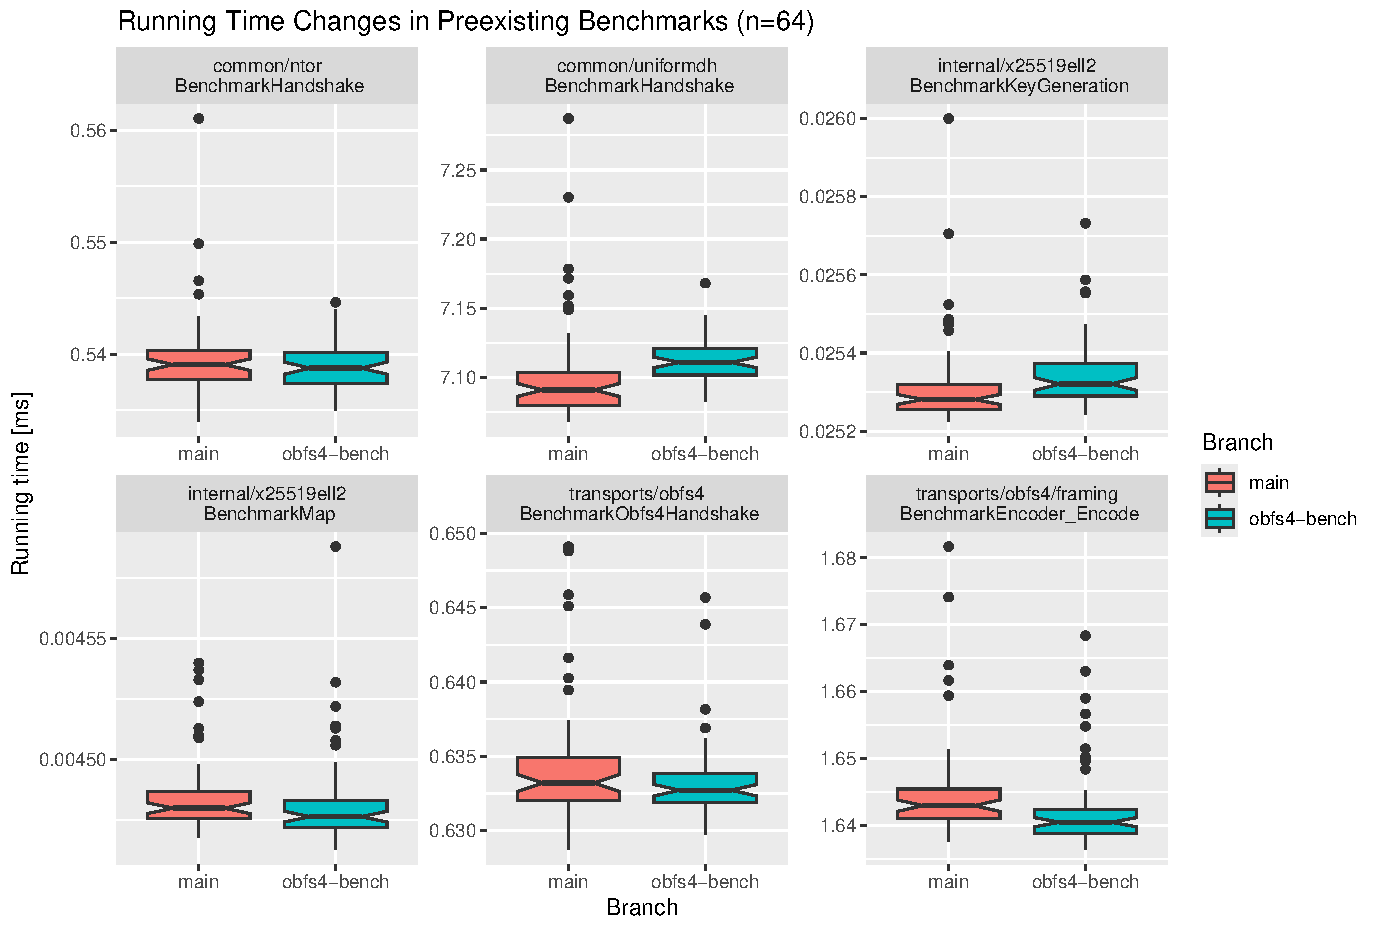
\includegraphics[width=0.9\linewidth,page=1]{images/Rplots.pdf}
    \noindent\rule{\linewidth}{0.4pt}
    \includegraphics[width=0.9\linewidth,page=2]{images/Rplots.pdf}
    \caption[
        Running Time and Memory Usage Changes in Preexisting Benchmarks.
    ]{
        Running Time and Memory Usage Changes in Preexisting Benchmarks.
        The x-axis denotes the branch in which the benchmark was run.
        Each panel denotes a specific benchmark available in both branches.
        The y-axis of the top plot shows performance in milliseconds per benchmark iteration.
        The y-axis of the bottom plot shows memory usage in total number of bytes allocated per benchmark iteration.
        The distribution of results is shown with notched boxplots \cite{mcgill-notched-boxplots}, where the box ranges from the 25\% to the 75\% quartiles, vertical ``whiskers'' show 1.5 times the height of the box, outside of which data points are ``outliers'' and drawn as dots.
        Notches in the sides of the box represent a roughly 95\% confidence interval, i.e.~if the notches of two boxes do not overlap, then this suggests that the medians are likely significantly different.
    }
    \label{fig:plot-1}
\end{figure}

\paragraph{Quantum-Safety at the Cost of Increased Time and Memory}

We now move to examine the benchmark results of simulated handshakes in particular.
That is, we compare the running time and memory usage of the \texttt{BenchmarkDrivelHandshake}, using each of our \drivel{} parameter sets defined in \cref{tab:drivel-params}, to the preexisting \texttt{BenchmarkObfs4Handshake} benchmark.

In each case, an interaction between a fictional client and a bridge server is played out and checked for correctness. The running time thus represents the combined cost of a handshake for both the client and the bridge server.

\Cref{fig:plot-3} shows the running time and memory usage of the simulated handshakes using the different bridge configurations.

We observe that our implementation has higher performance costs in both running time and memory usage compared to \obfsfour{}: The running time increase ranges from approximately a factor of 2 (for L0 security) up to a factor of almost 80 (for L5c using ML-KEM-1024 and FEO-HQC-256). The memory usage growth is even more pronounced, ranging from $12\times$ (for L0 security) up to $211\times$ (for L5b using BIKE-L5 and ML-Kemeleon-1024).

We attribute these results in part to the reasonably optimized implementation of \obfsfour{}, and further work on our implementation could surely decrease these numbers --- especially for L0 security, where one could expect comparable performance to \obfsfour{}. Additionally, some optimizations we propose later in \cref{sssec:variant-framing} might further reduce this difference.
However, it is also clear that increased resistance against quantum computers often comes at a cost to performance, and ultimately this cost must be weighed against the risk of compromise.

Differences between the different parameter sets stem directly from the implementation of the KEM, OKEM and filter-encode obfuscator (if any). These visualizations may help bridge operators when choosing which parameter sets to configure.

\begin{figure}[H]
    \centering
    \includegraphics[width=0.9\linewidth,page=3]{images/Rplots.pdf}
    \noindent\rule{\linewidth}{0.4pt}
    \includegraphics[width=0.9\linewidth,page=4]{images/Rplots.pdf}
    \caption[
        Simulated Handshake Running Time and Memory Usage.
    ]{
        Simulated Handshake Running Time and Memory Usage.
        The x-axis denotes the key exchange scheme in use for a benchmark, the axis is sorted according to parameter sets from \cref{tab:drivel-params}.
        Each panel denotes a pluggable transport, but \drivel{} measurements are further split by the targeted NIST security level (L0 representing that the configuration is not quantum-safe).
        The y-axis of the top plot shows performance in milliseconds per handshake.
        The y-axis of the bottom plot shows memory usage in total number of bytes allocated per benchmark iteration.
        Colors are used as a purely visual aid to identify similar KEM/OKEM combinations.
        No indications of measurement variance are present, as the maximum standard deviation observed in any parameter set is 0.342 milliseconds in the top plot and 15~534 bytes for the bottom plot.
    }
    \label{fig:plot-3}
\end{figure}

\newpage
\paragraph{KEM and OKEM Performance Matches Expectations}

Next, we examine the performance benchmarks of individual KEMs and OKEMs provided by our \texttt{internal/cryptofactory} module.

These benchmarks examine one of three operations: key generation, encapsulation (reusing the same randomly chosen public key) or decapsulation (reusing a public key and ciphertext from encapsulation).

\Cref{fig:plot-5} shows the running time and memory usage of these operations for each KEM.

In addition to our own benchmarks run in Go via our module, we include independent measurements of the KEM operations' running time taken from the SUPERCOP~\cite{supercop} project in the plots.
Our KEM implementations ultimately use the \texttt{liboqs} C library, and we compare our benchmarks with the corresponding measurements of the same KEMs and operations, where available.

To improve the comparability of the results, we use only a subset of SUPERCOP results, namely, the runs of three machines with a similar instruction set architecture to our infrastructure: One Skylake machine\footnote{See \url{https://bench.cr.yp.to/results-kem/amd64-samba.html}.} and two Coffee Lake machines\footnote{See \url{https://bench.cr.yp.to/results-kem/amd64-cubi10.html} and \url{https://bench.cr.yp.to/results-kem/amd64-know.html}.}.

We observe in \cref{fig:plot-5} that our Go module does not systematically add an overhead to the running time of the KEMs, as our numbers are not far off from the SUPERCOP measurements.

A notable exception is the HQC KEM, where we observe a $30\times$ longer running time. A more detailed look employing Go's profiling functionality confirmed that at least 95\% of our benchmark time is spent in \texttt{liboqs} code. We believe that the difference can be attributed to optimizations of the HQC code between our \texttt{liboqs} release (which claims to implement the Round 3 version of HQC) and the SUPERCOP measurements (using a Round 4 implementation).

Additionally, our filter-encode obfuscator for HQC does not have a significant impact on the total running time, although the public key filtering can be observed in the increased time for key generation (depending on the parameter set).
Our unoptimized implementation of Kemeleon severely degrades ML-KEM performance due to our focus on correctness first and foremost. However, our FEO-ML-KEM OKEMs still have running times comparable to those of HQC and FrodoKEM.

Memory usage shows patterns similar to running time, but emphasizes the potential for optimization in our Kemeleon implementation even more.

\begin{figure}
    \centering
    \includegraphics[width=0.9\linewidth,page=5]{images/Rplots.pdf}
    \noindent\rule{\linewidth}{0.4pt}
    \includegraphics[width=0.9\linewidth,page=6]{images/Rplots.pdf}
    \caption[
        (O)KEM Running Time and Memory Usage.
    ]{
        (O)KEM Running Time and Memory Usage.
        The x-axis denotes the KEM scheme in use for a benchmark, the axis is sorted according to the targeted NIST security levels.
        Each panel denotes a KEM family and is split into unobfuscated (``-'') and obfuscated variants (``FEO''), if both are implemented.
        The y-axis in the top plot shows the running time per KEM operation on a log scale.
        The y-axis in the bottom plot shows the memory usage in total number of bytes allocated per KEM operation on a log scale.
        Color indicates the KEM operation, and shapes indicate whether a measurement comes from our benchmarks or from SUPERCOP~\cite{supercop}. No SUPERCOP~\cite{supercop} measurements are available for memory usage.
        No indications of measurement variance are present, as the standard deviation would not be visible.
    }
    \label{fig:plot-5}
\end{figure}

\subsection{Deployment Results}

\paragraph{Overall Traffic Pattern is Similar to \obfsfour{}}

Using our Docker deployments, we were able to collect traffic captures from the virtual network. Using this data, we can visualize the overall network pattern.

\Cref{fig:plot-7} shows the traffic bandwidth used in slices of 100 milliseconds and attributes each packet to one a type depending on the communication peer and whether or not the packet is used for the pluggable transport handshake.

Our data shows that the general pattern of data bursts every second, which is created by the Tor protocol, constitutes the main traffic pattern in our experiments.
The handshake packets increase in size, while all other packet types use roughly the same bandwidth --- except for the initial burst of Tor traffic, which seems to take up more bandwidth in \obfsfour{} than in any \drivel{} configuration. The reason for this is unknown to us, as this traffic originates in the Tor software itself and not in the pluggable transport.

\begin{figure}
    \centering
    \includegraphics[width=0.9\linewidth,page=7]{images/Rplots.pdf}
    \caption[
        Network Traffic over Time.
    ]{
        Network Traffic over Time.
        The x-axis denotes the time in seconds since the first packet belonging to the test was observed.
        Each panel denotes a pluggable transport protocol, and values from \drivel{} configurations are averaged over all parameter sets from \cref{tab:drivel-params}.
        The y-axis shows the bandwidth usage in kilobits per second and is scaled in the same way for both protocols, negative values indicate ``downstream'' traffic from the bride to the client while positive values indicate ``upstream'' traffic originating at the client.
        Color indicates the packet type.
    }
    \label{fig:plot-7}
\end{figure}

\paragraph{Handshake Traffic Shows Expected Delays Due to (O)KEM Operations}

Zooming in on just the handshake packets (i.e.~the packet type colored blue in \cref{fig:plot-7}), we now want to examine the exact timing and bandwidth used by the key exchange.

\Cref{fig:plot-8} shows only the traffic bandwidth used for key exchange in slices of 1 millisecond and attributes each packet to its \drivel{} parameter set from \cref{tab:drivel-params} to better show the differences. The total number of bytes for key exchange sent over the course of any given deployment is shown on the side.

Besides the size differences in the various parameter sets, we can also observe the delay in the bridge response for the ``c'' parameter sets in particular.
These delays match our expectations from \cref{fig:plot-3}, as half of the simulated handshake running time in that plot is very close to the observed response delay here. This can in turn be explained by the high running time cost of HQC decapsulation as shown in \cref{fig:plot-5}.

Our fragmentation approach presented below in \cref{sssec:variant-framing} would also not protect against this delay, however, as the OKEM decapsulation is still required before a response can be sent. Bridge operators who are concerned about this, might want to consider alternative parameter sets, and future work might consider optimizing the HQC performance to more closely match the numbers from SUPERCOP.

\begin{figure}
    \centering
    \includegraphics[width=0.9\linewidth,page=8]{images/Rplots.pdf}
    \caption[
        Traffic for Key Exchange.
    ]{
        Traffic for Key Exchange.
        The x-axis denotes the time in milliseconds since the first packet belonging to the test was observed.
        Each panel denotes a pluggable transport, but \drivel{} measurements are further split by the targeted NIST security level (L0 representing that the configuration is not quantum-safe).
        Colors are used to indicate different parameter sets from \cref{tab:drivel-params}, which are also shown on the side.
        The y-axis in the left panels shows the bandwidth usage of data for the key exchange in kilobits per second, and values from different parameter sets are stacked.
        The y-axis in the right panels shows the total traffic volume of the key exchange objects in bytes, and values from different parameter sets are stacked.
        In all panels, negative values indicate ``downstream'' traffic from the bride to the client while positive values indicate ``upstream'' traffic originating at the client.
    }
    \label{fig:plot-8}
\end{figure}

\paragraph{Handshake Packets grow beyond fragmentation limits}

Finally, we analyze the observed packet sizes in terms of their TCP payload lengths and dive into the sizes of different components of the handshake packets.

\Cref{fig:plot-9} shows the size distribution of all TCP payloads by packet type and pluggable transport configuration, zooming in on only the handshake packets on the side.
\Cref{fig:plot-10} visualizes the sizes of the different components of the handshake packets, most notably the OKEM ciphertext, the encrypted KEM public key and the encrypted KEM ciphertext.
As the range of field sizes is quite large, \cref{fig:plot-10} also shows the same data using a logarithmic y-axis to allow more details to be visible.

Both \cref{fig:plot-9,fig:plot-10} include informational dotted lines showing packet size limits.
In a real-world setup, TCP payload sizes are effectively limited by the Maximum Transmission Unit (MTU) of the network. Beyond this limit, TCP packets are fragmented and transmitted as multiple smaller packets. This limit is shown in blue.
For our virtualized deployments, Docker relies on an OS functionality called Generic Segmentation Offload (GSO), i.e.~Docker containers may create TCP packets much larger than the MTU, and the OS will take care of further fragmentation, if needed. In our case, the packets never cross a physical link and are thus kept at their large original size.
We have determined that our setup allows for a maximum TCP payload size of 7~240 bytes; this limit is shown in red.
Note that \cref{fig:plot-9} also takes TCP headers into account, while \cref{fig:plot-10} works with payload sizes directly.

\Cref{fig:plot-9} shows that while the general size distribution of packets in our deployments remains roughly the same in \drivel{} compared to \obfsfour{}, as expected, handshake packets become significantly larger.

In particular, \cref{fig:plot-10} shows that almost all \drivel{} parameter sets exceed the MTU limit in their first message, and some even exceed the GSO limit. This will effectively cause TCP fragmentation for handshake messages, a feature which may be identifiable on the network layer as multiple maximally sized TCP packets are sent.

It should be noted that this MTU limit was already routinely exceeded for \obfsfour{} since padding can increase the payload size to up to 8~192 bytes, which would cause the transmission of up to five MTU-sized TCP packets (assuming a typical MTU of 1~500 bytes, i.e.~without using so-called ``Jumbo frames''). With \drivel{}, this phenomenon is even more pronounced.

A possible remedy for this issue could be to implement some fragmentation already within lyrebird, thus sending multiple packets with sizes below the MTU instead of relying on the OS to fragment messages. Although it is worth pointing out that the main contribution to the first message's size is often the OKEM ciphertext, and even with the optimizations discussed below in \cref{sssec:variant-framing}, MTU is quickly exceeded in this application.

\begin{figure}
    \centering
    \includegraphics[width=0.9\linewidth,page=9]{images/Rplots.pdf}
    \caption[
        Distribution of all TCP Packet Sizes.
    ]{
        Distribution of all TCP Packet Sizes.
        The x-axis denotes the TCP packet size in bytes (including the TCP header) and uses a log scale; the data is binned into 10 groups per tick on the x-axis.
        Each panel denotes a pluggable transport, but \drivel{} measurements are further split by the targeted NIST security level (L0 representing that the configuration is not quantum-safe), and values from different \drivel{} parameter sets are averaged per NIST security level.
        Color indicates the packet type.
        The right panels show the same data but filtered only on packets of type ``handshake (bridge)''.
        The y-axis in the left panels shows the frequency of a given size in percent of all recorded packets, and values from different packet types are stacked.
        The y-axis in the right panels shows the frequency of a given size in percent of all handshake-type packets.
        The blue dotted line denotes the a typical MTU limit of 1~500 bytes, while the red dotted line shows our effective TCP packet size limit of 7~280 bytes using Generic Segmentation Offload.
    }
    \label{fig:plot-9}
\end{figure}

\begin{figure}
    \centering
    \includegraphics[width=0.9\linewidth,page=10]{images/Rplots.pdf}
    \noindent\rule{\linewidth}{0.4pt}
    \includegraphics[width=0.9\linewidth,page=11]{images/Rplots.pdf}
    \caption[
        Composition of Handshake Packets.
    ]{
        Composition of Handshake Packets.
        The x-axis denotes the packet's origin using the Docker container names.
        Each panel denotes a pluggable transport, but \drivel{} measurements are further split by the targeted NIST security level (L0 representing that the configuration is not quantum-safe), and split again into each \drivel{} parameter set from \cref{tab:drivel-params}.
        Color indicates the protocol field whose size is displayed.
        The y-axis shows the size of the different protocol fields in bytes, and values from different fields are stacked.
        The blue dotted line denotes the a typical TCP payload limit of 1~460 bytes (corresponding to a MTU of 1~500 bytes), while the red dotted line shows our effective TCP payload size limit of 7~240 bytes using Generic Segmentation Offload. These values differ from \cref{fig:plot-9} as we ignore TCP headers here.
    }
    \label{fig:plot-10}
\end{figure}

\newpage
\section{Conclusions} \label{sec:conclusion}

In this chapter, we presented our experimental process, showed our results, and interpreted the data. In summary:
\begin{itemize}
    \item Our implementation of \drivel{} integrates nicely into the lyrebird repository and does not affect the performance of other pluggable transports implemented.

    \item Our newly added crypto-agile framework implementing KEMs and OKEMs performs as expected when compared with SUPERCOP benchmarks. The only exception to this is the HQC KEM, which performs worse than SUPERCOP by a factor of about $30\times$ in our measurements. Notably, different versions of HQC were used in our implementation versus the SUPERCOP benchmarks.

    \item While \drivel{} provides higher security guarantees than \obfsfour{}, and, in particular, achieves security against quantum computers when instantiated with appropriate (O)KEMs; this comes at the cost of an increase in running time of up to $80\times$ and a higher memory usage of up to $211\times$, depending on the concrete parameter set chosen.

    \item Our benchmarks give an accurate picture of the performance observed in our deployments in terms of latency, allowing developers to have a realistic idea of the performance without carrying out a deployment.

    \item The main difference in traffic patterns is the larger size of handshake packets, which could be identified by censors, emphasizing the need for fragmentation functionality within the obfuscated key exchange protocol itself.

    \item Finally, our parameter sets offer a range of trade-offs between security, running time (i.e.~latency) and memory usage, which may aid bridge operators in selecting a suitable configuration.
\end{itemize}
